\begin{figure}
    \centering
    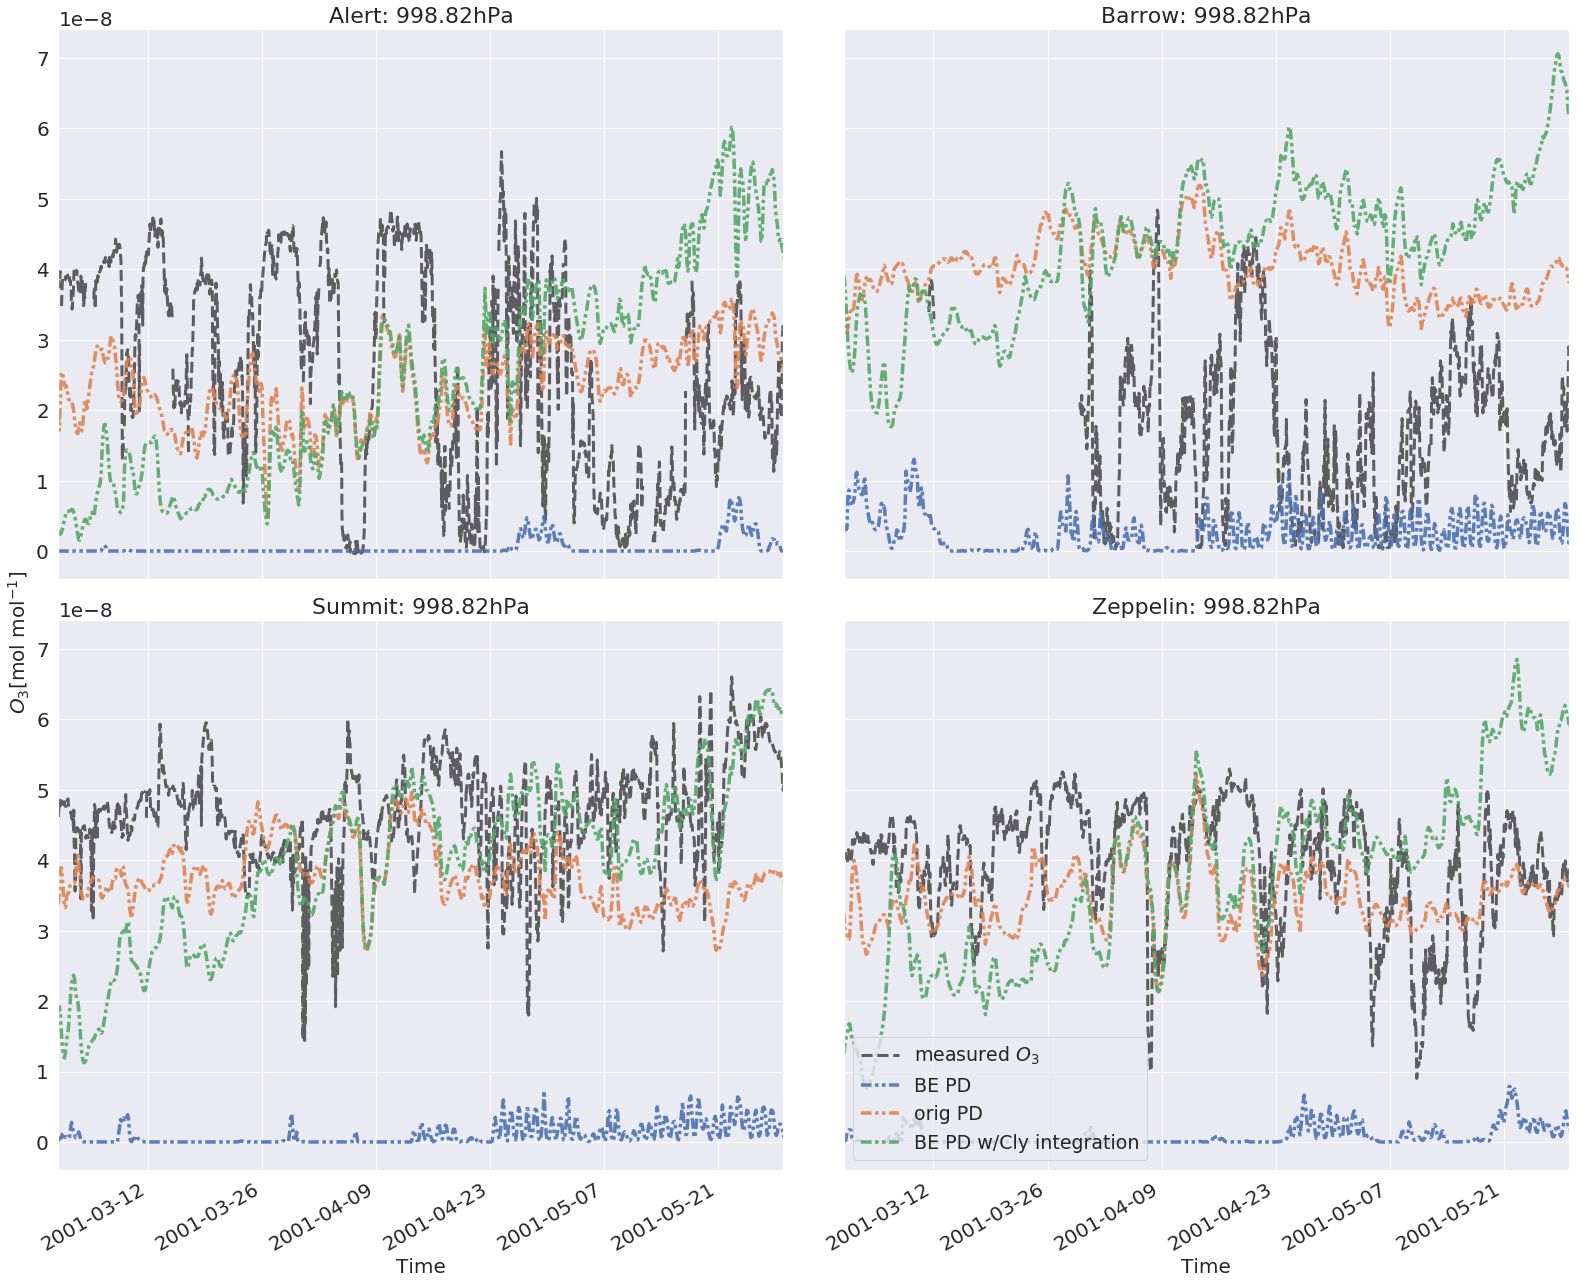
\includegraphics[width = \linewidth]{Chapter6_Results/images/ozone_2001_newClyIntegration.png}
    \caption{Ozone measurements (black line) and model results from the original CTM3 (orange line), Branch \ref{def:BE_PD} (blue line) and the attempt to integrate the $\chem{Cl_y}$ family (green line) at the four different stations, Alert (top left), Barrow (top right), Summit (lower left) and Zeppelin (lower right) with available measurements in 2001. Model results are taken from the first model level at $998.82 hPa$. PD = present day, BE = bromine explosion}
    \label{fig:test_ClyInt}
\end{figure}